\documentclass{beamer}
\usetheme{Berlin}

\usepackage{graphicx}
\usepackage{wrapfig}
\usepackage[ngerman]{babel}
\usepackage[utf8x]{inputenc}

\usepackage{todonotes}
\presetkeys{todonotes}{inline}{}

\begin{document}

\let\todox\todo
\renewcommand\todo[1]{\vspace{0.3em}\todox[inline, size=\small , color=red!20]{#1}}

\title{Performanz Evaluation von Graphdatenbanksystemen versus MySQL am Beispiel von Kookkurrenzgraphen}
\author{Martin Junghanns, Sascha Ludwig \& Robert Schulze} 
\date{\today}
\logo{
\includegraphics[scale=0.14]{uni_leipzig_logo}}
\setbeamertemplate{navigation symbols}{}

\begin{frame}
	\titlepage
\end{frame}

\begin{frame}\frametitle{Inhalt}
	\tableofcontents
\end{frame}

\section{Einleitung}

\begin{frame}\frametitle{Aufgabenstellung}
	\begin{itemize}
		\item Evaluation verschiedener Graphdatenbanken
		\item Gegenüberstellung mit einer relationalen Datenbank
		\item Datenbasis des Wortschatz Leipzig Projekts
		\item Implementierung eines Frameworks zur Durchführung von Benchmarks in Java
		\item Auswertung und Visualisierung der Messergebnisse
	\end{itemize} 
\end{frame}

\begin{frame}\frametitle{Graphdatenbanken --- allgemein}
	\begin{itemize}
		\item Datenmodellierung als Graph
		\item Vermeidung von Verbundoperation
		\item Schemafreiheit
		\item Anwendung: Soziale Netzwerke, Recommendation, Transportnetze
	\end{itemize} 
\end{frame}

\begin{frame}\frametitle{Graphdatenbanken --- Auswahl}
	\begin{description}
		\item[Neo4j] gute Skalierbarkeit, Traversal-Framework, geringe Speicheranforderungen
		\item[OrientDB] Feature-Vielfalt: SQL-Abfragesprache; Embedded oder als Server
		\item[DEX] Backend in C++ mit Java-API; gilt als performanteste Graphdatenbank auf dem Markt
	\end{description}
\end{frame}

\begin{frame}\frametitle{Schemavergleich}
\begin{figure}[ht]
\begin{minipage}[b]{0.45\linewidth}
\centering
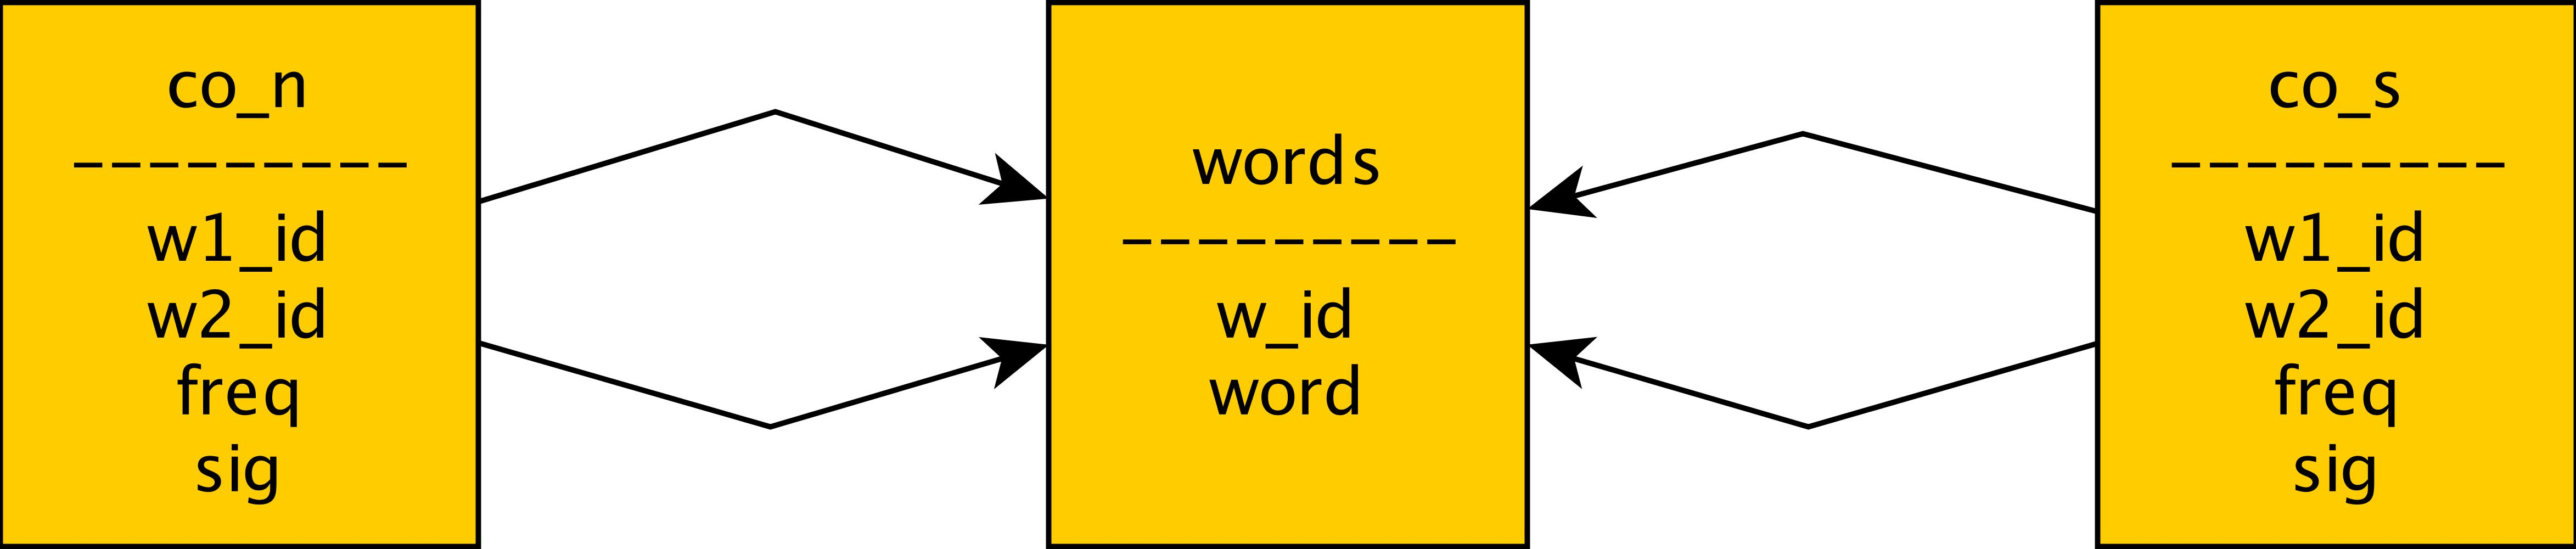
\includegraphics[scale=0.03]{images/mysql_schema}
\caption{Mysql Schema}
\label{fig:mysql_schema}
\end{minipage}
\hspace{0.5cm}
\begin{minipage}[b]{0.45\linewidth}
\centering
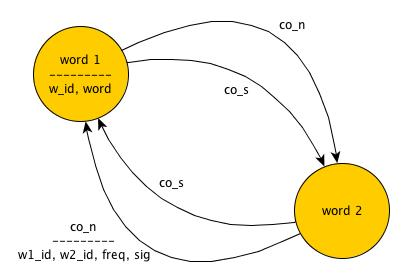
\includegraphics[scale=0.1]{images/graph_schema}
\caption{Graph}
\label{fig:graph_schema}
\end{minipage}
\end{figure}
\end{frame}

\begin{frame}\frametitle{Testdaten}
	\begin{table}
	\begin{tabular}{|l|r|r|r|}
		\hline
		Datenbank & Knoten & \multicolumn{2}{|c|}{Kanten}\\
		\hline
		 & words & co\_{}s & co\_{}n \\
		\hline
		\hline
		deu\_{}news\_{}2009\_{}10K & 39334 & 22062 & 5887\\
		\hline
		deu\_{}news\_{}2009\_{}100K & 191041 & 297422 & 69297\\
		\hline
		deu\_{}news\_{}2009\_{}300K & 390178 & 953218 & 196122\\
		\hline
		deu\_{}news\_{}2009\_{}1M & 830641 & 3349314 & 584402\\
		\hline
		deu\_{}news\_{}2009\_{}3M & 1623621 & 10596746 & 1546638\\
		\hline
		deu\_{}news\_{}2009\_{}10M & 3309332 & 37393614 & 4412321\\
		\hline
	\end{tabular}
	\caption{Kookkurrenzgraph des Wortschatz Leipzig}
	\end{table}
\end{frame}

\begin{frame}\frametitle{Queries erklären}
\begin{description}
\item[Query 1]Finde alle Satz- oder Nachbarschaftskookkurrenzen eines Wortes. Gib Frequenz, Signifikanz und die beteiligten Wörter der Kookkurrenz aus.
\item[Query 2]Finde alle Satz- oder Nachbarschaftskookkurrenzen der Nachbarn eines Wortes. Gib Frequenz, Signifikanz und die beteiligten Wörter der Kookkurrenz aus.
\item[Query 3]Finde alle Satz- oder Nachbarschaftskookkurrenzen zwischen den Nachbarn eines Wortes. Gib Frequenz, Signifikanz und die beteiligten Wörter der Kookkurrenz aus.
\end{description}
\end{frame}

\section{Durchführung}
\begin{frame}\frametitle{Framework} 
	\begin{itemize}
		\item Verbindung zur Datenbank
		\item Importieren von Datenbasis aus MySQL
		\item Durchführung einzelner Benchmarks und Messung durchschnittlicher Ausführungszeiten von Datenbankoperationen
		\item Konfiguration über Java-properties-Dateien
	\end{itemize} 
\end{frame}

\section{Auswertung}
\begin{frame}\frametitle{Auswertung}
	\begin{itemize}
		\item 
		\item 
		\item 
	\end{itemize} 
\end{frame}

\begin{frame}\frametitle{} 
	\begin{itemize}
		\item 
		\item 
		\item 
	\end{itemize} 
\end{frame}

\begin{frame}
	\begin{center}
		\begin{Huge}
			Ende
		\end{Huge}
	\end{center}
\end{frame}

\end{document}